\section{Metadata}
The metadata contains all the information \emph{about} the data, such as conversion parameters, but also filter and plot parameters. The package comes shipped with `default' parameters, which can be used when the data is first imported by the user. It is recommended to copy the default parameters close to the local files, such that they are not changed, for instance when the package is upgraded.
The default metadata in the package is defined for each spectrometer, since each spectrometer has different numbers of detectors, with different measurement signals (position, time, etc \dots). 

\begin{figure}[H]
   \centering
    \centerline{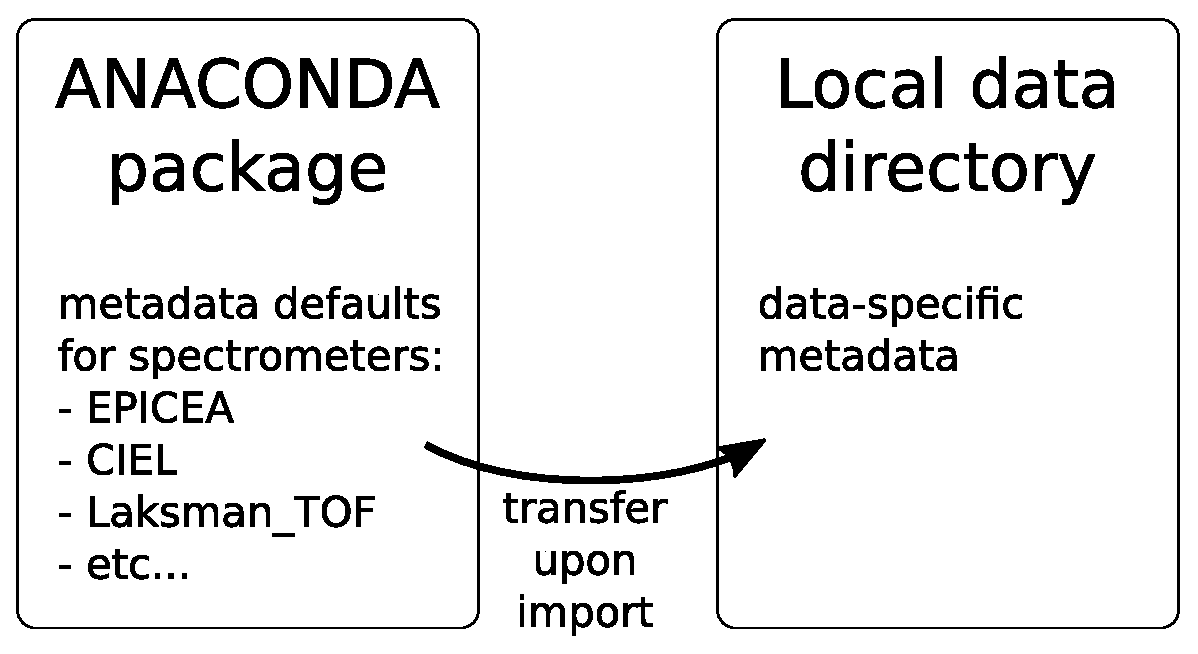
\includegraphics[width=0.7\textwidth]{Graphics/metadata_defaults.eps}}
\caption{Default metadata (or configuration data) are defined in the package, to be copied upon first import of a new data file.}
\label{metadata_defaults}
\end{figure}

\subsection{Metadata structure}
The metadata contains all information needed to correct, convert, fit and visualize the data.
\\
The metadata structure is divided into different categories:
\begin{itemize}
\item[\emph{sample}], e.g. atomic mass, expected fragment masses, constituent masses.
\item[\emph{photon beam}], e.g. the photon energy, intensity, duration, etc
\item[\emph{spectrometer}],  e.g. the name, voltages and relevant dimensions of the used spectrometer are listed here.
\item[\emph{detectors}], e.g. the names and properties of the detectors are stored in here.
\item[\emph{correct}] The parameters needed to execute corrections onto the raw data, before conversion. For example, translation in X and Y to move the centre of detection into the origin of the coordinate system.
\item[\emph{calibrate}] The information needed to perform the calibrations. Note that these are not the actual calibration factors, they are stored in the 'convert' field.
\item[\emph{fit}] The fitting parameters.
\item[\emph{convert}] The conversion factors (sorted in terms of detectors), such as mass to charge conversion.
\item[\emph{plot}] The user-preferred plotstyle.
\end{itemize}

Most fields in the metadata are obvious to understand. We elaborate on a few that might be cause of confusion.

\paragraph{sample}
 We elaborate on the definition difference between 'constituents' and 'fragments' here:
\begin{itemize}
\item Constituents: The building block of which the sample consists. Example: a water-ammonia mixed cluster has consituents water and ammonia
\item Fragments: The expected fragments from the sample. Example: a water-ammonia mixed cluster has the expected fragments of hydrogenated water-ammonia mixed clusters.
\end{itemize}


\subsection {storage}
The metadata is stored as a struct, with the above categories as their fieldnames. 

The metadata, or data settings, belong to a separate datafile. They are stored in a separate file with the same base name as the main datafile (\emph{'filename.mat'}), but with the addition \emph{'md\_.m'} before the filename, so \emph{'md\_filename.m'}. This is done to make it easy to manually copy metadata files to different datafiles. For example: reading the datafile \emph{H2O\_003.mat} will read its metadata from the file \emph{md\_H2O003.m}. The metadata is stored in a plain-text m-file, which makes it possible to read and change parameters from outside MATLAB.

\lstset{language=MATLAB}
\begin{lstlisting}
exp1_md.sample
exp1_md.photon
exp1_md.spec
exp1_md.corr
exp1_md.calib
exp1_md.fit
exp1_md.conv
exp1_md.plot
\end{lstlisting}
